\chapter{Estado del arte}\label{Chapter2} 
\section{Conservación de procedimiento científicos}

Distintas áreas de la ciencia han adoptado técnicas y herramientas para conservar el procedimiento. Por ejemplo, investigadores en bio-informática ha incorporado los workflows para distintos análisis: 
Doblamiento de proteínas \cite{craddock2006science}, secuencias de DNA y RNA \cite{blankenberg2010galaxy,giardine2005galaxy} y la detección de ondas gravitacionales \cite{deelman2004pegasus}.
Los workflows científicos son métodos que permiten representar un conjunto de pasos computacionales. Estos pasos pueden ser la obtención de los datos de entrada, transformaciones o generación de los resultados.
La representación de los workflow se construye en un lenguaje abstracto para simplificar la complejidad. El conjunto de pasos se pueden representar como gráfos sin ciclos y dirigidos, donde cada paso computacional es representado por un nodo y las dependencias entre los pasos son representado por los arcos.
El uso de sistemas de manejo de workflows científicos \textit{Scientific Workflow management Systems (WMS)} permiten diseñar abstractamente, ejecutar y compartir el procedimiento científicos. 

Dado que los workflows formalmente describen la secuencia de tareas computacionales y administración de datos, es fácil encontrar el camino de los datos producidos.
Un científico podría ver el workflow y los datos, seguir los pasos y llegar al mismo resultado. En otras palabras, la representación del workflow facilita la creación y administración de la computación y además construye una base en la cual los resultados pueden ser validados y compartidos.

Sin embargo, múltiples estudios han mostrado las dificultades reproducir los resultados de los experimentos.

%todo: ampliar estos


%Como se menciono, la mayoría de las propuestas de reproducibilidad de ambientes en las ciencias de computación se han enfocado en los datos, el código y la descripción de workflow pero ha dejando de lado los recursos computacionales y componentes de software. Siendo un recurso esencial para reproducir el experimento

%De acuerdo a \cite{king1995replication}, en orden de reproducir o replicar un artefacto digital es necesario manejar su conservación y para alcanzar esta conservación se debe garantizar que: existe la suficiente información con la cual se pueda entender, evaluar y construir un trabajo anterior sin información adicional del autor. 

%Uno de los trabajos que se ha enfocado en conservar los recursos de un ambiente computacional es \cite{santana2017reproducibility}. Donde los autores han identificado dos enfoques para conservar un ambiente científico. Conversación física: donde el objeto real es conservado dada la relevancia y la dificultada de obtener una replica y  Conversación lógica: donde los objetos son descriptos en una manera que un experimento similar puede ser obtenido en un futuro experimento.


\subsection{Sistemas de administración de workflows}

Cómo se menciono anteriormente, los workflows científicos permiten a los usuarios expresar fácilmente tareas computacionales de varios pasos, por ejemplo, recuperar datos de un instrumento o una base de datos, reformatear los datos y ejecutar un análisis. 
Un workflow científico describe las dependencias entre las tareas y la mayoría de los casos se describe como un gráfico acíclico dirigido (DAG), donde los nodos son tareas y los bordes denotan las dependencias de las tareas.
Una propiedad que define un workflow científico es que gestiona el flujo de datos. Es por ello, que las tareas en un  workflow científico varían ampliamente según las necesidades del autor, los tipos pueden ser tanto como tareas cortas en serie o tareas paralelas muy grandes (e.g, utilizando Message Passing Interface - MPI) rodeadas de un gran número de pequeñas tareas en serie utilizadas para el pre y post procesamiento.
La interpretación y ejecución de los workflows son manejados por un sistema de manejo de workflows (WMS) que administra la ejecución de la aplicación en la infraestructura. 
Un WMS puede ser considerado como una capa intermedia necesaria para la abstracción y orquestación de procedimiento científico. A continuación se describe algunos de los WMS más populares.

Actualmente, existen múltiples WMS que han sido generado por diversas comunidades.
\subsection{Galaxy}	
%todo: mejorar esto
Galaxy \cite{goecks2010galaxy} es un sistema de gestión de almacenes basado en la web que tiene como objetivo llevar las capacidades de análisis de datos computacionales a usuarios no expertos en el campo de las ciencias biológicas. Los principales objetivos del marco de trabajo de Galaxy son la accesibilidad a las capacidades computacionales biológicas y la reproducibilidad del resultado del análisis mediante el seguimiento de la información relacionada con cada paso del proceso. 
%todo: mejorar esto
\subsection{Taverna}	
Taverna \cite{DBLP:journals/bioinformatics/OinnAFMSGCGPWL04} es un WMS basado en servicios web, ya que todos los componentes del flujo de trabajo deben implementarse como servicios web (ya sea localmente o utilizando un servicio remoto disponible). Taverna es capaz de integrar los servicios web de Soaplab26, REST (Fielding, 2000) y WSDL (Christensen et al., 2001). Ofrece una amplia gama de servicios para diferentes capacidades de procesamiento, tales como servicios Java locales, servicios de procesador R estadístico, scripts XPath o servicios de importación de hojas de cálculo.
%todo: mejorar esto
\subsection{Pegasus}
Pegasus \cite{deelman2004pegasus} es un WMS capaz de gestionar flujos de trabajo compuestos por millones de tareas, registrando datos sobre la ejecución y resultados intermedios. En Pegasus, los flujos de trabajo se describen como flujos de trabajo abstractos, que no contienen información de recursos, o las ubicaciones físicas de datos y ejecutables.
%todo: mejorar esto
\subsection{WINGS} 
WINGS \cite{DBLP:journals/expert/GilRKGGMD11}  no puede ser considerado como un WMS apropiado por sí mismo, ya que no proporciona características de ejecución y promulgación del flujo de trabajo. Sin embargo, es ampliamente conocido por el diseño del flujo de trabajo. WINGS puede considerarse como una herramienta de diseño de alto nivel y orientada a los dominios, cuyos flujos de trabajo pueden ejecutarse posteriormente en diferentes motores de flujo de trabajo, como Pegasus o Apache OODT29.
%todo: mejorar esto
\subsection{dispel4py}
dispel4py \cite{DBLP:conf/eScience/FilgueiraKAKSS15}  es una biblioteca Python (Rossum, 1995) para describir flujos de trabajo. Describe flujos de trabajo abstractos para aplicaciones intensivas en datos, que luego se traducen y ejecutan en plataformas distribuidas (por ejemplo, Apache Storm, clusters MPI, etc.).

\section{Conservación de equipamiento}
Comúnmente el equipamiento en otras disciplinas no es un problema a resolver dado que los recursos utilizados son son conocidos, no-variables y estándares. Por ejemplo, la utilización de probetas, microscopios u otros elementos físicos. 
Consecuentemente, los investigadores pueden nombrarlos e identificarlos de forma manual en los procedimientos de sus cuadernos de laboratorio. Lo que permite que otro investigador conozca cuáles fueron las herramientas utilizadas en el experimento.
Aunque existen excepciones como en la ciencia de biología, donde ciertos recursos son materiales que son utilizados en los procedimientos. En estos casos, los investigadores deben describir los materiales incluyendo información como marcas, composición y otros. 
En otras ciencias cómo la astronomía se utilizan recursos  de alta tecnología, donde también es necesario documentar las características de hardware y configuraciones utilizadas en el proceso experimental. 
En las ciencias de la computación sucede un caso similar, dado que los recursos computacionales son una componente requerida en la ejecución del sistema. 
Es por ello, que esta comunidad no puede ser la excepción respecto a la descripción de los recursos. Por lo tanto, los autores deben poder documentar computadores, clusters, servicios web, componentes de software, etc., en el contexto de sus experimentos.

Diversos trabajos han estudiado el estado actual de la reproducibilidad en las ciencias de computación, en \cite{DBLP:conf/eScience/ZhaoGBKGGHRRG12} se estudia el factor de decaimiento de un conjunto workflows científicos almacenado en myExperiment \footnote{\url{https://www.myexperiment.org/home}} que fueron diseñados para el WMS Taverna \cite{DBLP:journals/bioinformatics/OinnAFMSGCGPWL04} del área de biología. Para ello, los autores utilizaron cuatro conjuntos de paquetes de workflows y clasifican el decaimiento de los workflows en cuatro categorías: recursos de terceros volatiles, datos de ejemplos faltantes, ambiente de ejecución faltante y descripciones insuficientes sobre los workflow. El estudio muestra que casi el 80\% de workflows fallan al ser reproducidos, con un 12\% de esos fallos debido al ambiente de ejecución faltante y 50\% recursos de terceros volatiles. Estas dos últimas categorías están asociadas a la conservación del ambiente computacional del experimento.
En \cite{DBLP:conf/ipres/MatthewsCWJBS09}, los autores describen un procedimiento para preservar el software, argumentando que el software es frágil a los cambios de ambiente ya sea hardware, sistema operativo, versiones de las dependencias y configuración. Los autores afirman que el software no puede ser preservado con la metodología anterior de sólo mantener su código binario ejecutable. Por ello, introducen el concepto de adecuación de la preservación, una métrica para medir si la preservación de conjunto de funcionalidades de componente de software luego de un proceso reproducción.

De la misma manera, editoriales se ha enfocado en intentar resolver los desafíos en la publicación de trabajos científicos. Por ejemplo, Elsevier formó el \textit{Executable Paper Grand Challenge} para abordar la dificultad de reproducibilidad de los resultados en las ciencias de la computación, ellos  argumentan que los bloques vitales y necesarios de información para replicar los resultados -por ejemplo, software, código, grandes conjuntos de datos- no suelen estar disponibles en el contexto de una publicación académica. 
Y \textit{Executable Paper Grand Challenge} creó una oportunidad para que los científicos diseñen soluciones que capturen esta información y proporcionen una plataforma para que estos datos puedan ser verificados y manipulados. 
En 2011, \cite{DBLP:journals/procedia/BrammerCMW11} se argumenta que el documento de investigación en su estado actual ya no es suficiente para reproducir, validar o revisar completamente los resultados y conclusiones experimentales de un documento. Esto impide el progreso científico. 
Para remediar estas preocupaciones, presentan Paper Mâché, un nuevo sistema para crear documentos de investigación dinámicos y ejecutables. La principal novedad de Paper Mâché es el uso de máquinas virtuales, que permite a los lectores y revisores ver e interactuar fácilmente con un documento y poder reproducir los principales resultados experimentales.
En la misma línea, CernVM \cite{buncic2010cernvm} propuso la utilización de máquinas virtuales para resolver problemas de reproducibilidad en la ciencia. CernVM es un sistema para el uso de máquina virtuales capaz de ejecutar aplicaciones físicas de los experimentos relacionados al \textit{Large Hadron Collider} (LHC) en el \textit{European Organization for Nuclear Research} (CERN). Su objetivo es proporcionar un entorno completo y portátil para desarrollar y ejecutar el análisis de datos LHC en cualquier ordenador del usuario final (portátil, de sobremesa), así como en la red, independientemente de las plataformas de sistemas operativos (Linux, Windows, MacOS). La motivación del uso de técnicas de virtualización que permite separar los recursos de computación desde la infraestructura subyacente.

Algunos autores han expuesto la necesidad de capturar y preservar el entorno de ejecución de un ejecución del experimento, proporcionando herramientas para analizar y empaquetar los recursos involucrados en él.
ReproZip \cite{DBLP:conf/tapp/ChirigatiSF13} busca captar el conocimiento sobre una infraestructura e intentar reproducirla en un nuevo entorno. Esta herramienta lee los componentes de infraestructura involucrados en la ejecución (archivos, variables de entorno, etc.) y almacena esta información en una base de datos MongoDB \footnote{\url{https://www.mongodb.com/es}}. 
A continuación se recogen y empaquetan los elementos descritos. Luego, el sistema debe desempaquetar los elementos  en otra máquina para reproducir el experimento. Sin embargo, este tipo de enfoque que empaqueta los componentes físicos de una infraestructura determinada presenta limitación en la práctica, debido que los paquetes deben ser ejecutado en una máquina destino similar.
Otro ejemplo es TOSCA (Topology and Orchestration Specification for Cloud Applications), TOSCA es un ejemplo de las soluciones que han definido sintaxis para describir la ejecución de los ambientes computacionales. TOSCA es un lenguaje de código abierto utilizado para describir las relaciones y dependencias entre servicios y aplicaciones que residen en una plataforma de computación. TOSCA puede describir un servicio de computación en nube y sus componentes y documentar la forma en que están organizados y el proceso de orquestación necesario para utilizar o modificar dichos componentes y servicios. Esto proporciona a los administradores una forma común de gestionar aplicaciones y servicios en la nube, de modo que esas aplicaciones y servicios puedan ser portátiles a través de las diferentes plataformas de los proveedores de cloud computing. 
Otro esfuerzo importante relacionado a nuestro trabajo incluye la descripción de los ambientes computaciones utilizando ontologías es TIMBUS. El proyecto se focaliza en preservar procesos de negocios y su infraestructura computacional.  Para ello, propusieron un extractor para extraer y anotar los componentes de Software y Hardware, éstas anotaciones son almacenadas según un conjunto de ontologías con el objetivo de gestionar la preservación y reejecución de los procesos de negocio. Sin embargo, el enfoque extractor del Proyecto Timbus no es adecuado para ser utilizado en cualquier sistema de virtualizada ya que aumenta la complejidad del ambiente y generando ruido. Además, exige ejecutar el ambiente computacional lo cual conlleva altos costos computacionales, disminución en la escalabilidad y creación de brechas de seguridad. 

En el enfoque de describir los recursos computacionales, los autores en \cite{santana2017reproducibility} identificaron dos enfoques para conservar el  ambiente computacional de un experimento científico: la conservación física, donde los objetos de investigación dentro del experimento se conservan en un entorno virtual; y la conservación lógica, donde las principales capacidades de los recursos en el entorno se describen utilizando vocabularios semánticos para permitir al investigador reproducir un entorno equivalente. Para ello, definieron un proceso para documentar la aplicación de flujo de trabajo y su sistema de gestión relacionado, así como sus dependencias. Además, los autores propusieron \textit{The Workflow Infrastructure Conservation Using Semantics ontology} (WICUS). WICUS es una red de ontologías OWL2 (Web Ontology Language) que implementan la conceptualización de los principales dominios de una infraestructura computacional. Como: Hardware, Software, Workflow y Recursos Informáticos. 
Los autores argumentan este trabajo debido que a que el workflow científico requiere un conjunto de componentes de software, y los investigadores deben saber cómo desplegar esta pila de software para lograr un entorno equivalente.
Sin embargo, este proceso se realiza de forma de manual, dejando mucho trabajo a los científicos. 
Además, los autores afirman que la conservación de los ambientes computacionales comúnmente se logra utilizando un enfoque físico dado que la conservación física permite compartir fácilmente un ambiente computacional con otros investigadores y ellos pueden reproducir el experimento utilizando en el mismo ambiente. 
Sin embargo, los esfuerzos necesarios para mantener la infraestructura son altos y no hay garantías que no sufran un proceso de decaimiento \cite{DBLP:journals/fgcs/DeelmanVJRCMMCS15}.  
Consecuentemente, la mayoría de los trabajos dejan fuera del ámbito de aplicación la conservación física del entorno informático del workflow (basándose en la infraestructura elegida). Pese a que la conservación lógica y física son deseadas para lograr la reproducibilidad del experimento. 

En diversos trabajos ~\cite{DBLP:journals/bioinformatics/LeprevostGARUBV17, Beaulieu2017, Boettiger:2015:IDR:2723872.2723882, aranguren2015enhanced} se ha propuesto la utilización de Docker como un reemplazo al uso de máquinas virtuales como ambiente computacionales científicos, los trabajos argumentan que Docker presenta beneficios de portabilidad, documentación precisa de la instalación y configuración, manejo de control de versiones de las imágenes y fácil adopción por desarroladores. 
Un ejemplo de uso de Docker para la reproducibilidad es Biocontenedores \cite{DBLP:journals/bioinformatics/LeprevostGARUBV17}. Biocontenedores es un framework de código abierto y orientado a la comunidad que proporciona entornos ejecutables independientes de la plataforma para el software de bioinformática. Biocontenedores permite a los laboratorios instalar fácilmente software de bioinformática, mantener múltiples versiones del mismo software y combinar herramientas de análisis. Biocontenedores se basa en los populares proyectos de código abierto Docker~\footnote{\url{https://www.docker.com/}}, Singularity~\footnote{\url{https://www.sylabs.io/singularity/}} y rkt~\footnote{\url{https://coreos.com/rkt/}}, que permiten que el software sea instalado y ejecutado bajo un entorno aislado y controlado.
Sin embargo, en \cite{Boettiger:2015:IDR:2723872.2723882,DBLP:conf/semweb/OsorioAV18} los autores exponen que Docker no controla que paquetes instalados en las imágenes y no existe una descripción completa de los componentes de la imagen y consecuente del contenedor. Por lo tanto, las imágenes Docker funcionan como una caja negra, lo que significa que los usuarios saben cuál es el paquete que se ejecuta dentro del contenedor pero no conocen las versiones o los otros paquetes necesarios para ejecutarlo.

Respecto a la descripción de los componentes de una imagen Docker, en \cite{Shu:2017:SSV:3029806.3029832:DockerHub:Security} analizó más de 300.000 imágenes de Docker almacenadas en el repositorio oficial de Docker. Los autores encontraron que en promedio las imágenes que contiene el Docker Hub (sistema de almacenamiento de imágenes) son más de 180 vulnerabilidades, siendo la raíz de tal cantidad de vulnerabilidades el hecho de que muchas imágenes no han sido actualizadas en varios días y que muchas de estas vulnerabilidades se propagan de imágenes de padres a hijos. Los autores encontraron correlaciones entre las imágenes más influyentes y los paquetes vulnerables mejor clasificados, lo que sugiere que la fuente de esa cantidad de vulnerabilidades era probablemente el resultado de la propagación de un pequeño número de imágenes populares (debido a la falta de actualización de las imágenes principales). Los autores utilizaron el software Clair \footnote{\url{https://github.com/coreos/clair}} de la empresa CoreOS\footnote{\url{https://coreos.com/}}. 
En términos de ingeniería ontológica, los autores en~\cite{huo2015smart} presentan la ontología Smart contenedor que extiende DOLCE~\cite{gangemi2002sweetening} y modela Docker en términos de sus interacciones para desplegar imágenes. Otro trabajo relacionado, ~\cite{tommasini2017representing}  describe cómo usar RDF para representar archivos de construcción de Docker. 

\section{Docker}

Durante los últimos veinte años el uso de tecnologías de virtualización ha aumentado
	rápidamente, esta tecnología permite dividir el sistema de un computador
	en múltiples ambientes virtuales. 
	%Los importantes beneficios que entrega esta 	tecnología ha hecho que la virtualización sea muy utilizada \cite{bui2015analysis}.

Uno de los usos comunes para esta tecnología es la virtualización de 
	servidores en \textit{datacenters}. Con la virtualización de servidores, un
	administrador de sistemas puede crear una o más instancias virtuales o 
	máquinas virtuales (VMs) en un servidor. Este enfoque hoy se utiliza comúnmente en \textit{datacenters} y también en plataformas de \textit{cloud} como Amazon 	EC2, RackSpace, Dreamhost y otros \cite{felter2014updated}. 
El crecimiento del uso de la virtualización ha hecho necesario la búsqueda de una solución que permita tener un ambiente escalable y seguro. Un gran numero de
	soluciones han nacido en el mercado y se pueden clasificar en dos tipos:
	\textit{contenedor-based virtualization} y \textit{Virtualización basada en hipervisores}.
\textit{contenedor-based virtualization} es una virtualización liviana a
	nivel de software usando el kernel de host para correr múltiples ambientes virtuales.
Estos ambientes son nombrados con contenedores (contenedores).
	Y hoy en día Linux-VServer, OpenVZ, libcontenedor y Linux contenedor (LXC) son
	las principales implementaciones para utilizar contenedores. En la
	figura~\ref{fig:contenedor-arch} se puede observar que la arquitectura de
	\textit{contenedor-based virtualization}. Los contenedores utilizan el sistema	operativo compartido del ambiente virtualizador (host) y por lo tanto no es necesario nuevamente el sistema operativo para cada contenedores que se está ejecutado.
Para el sistema operativo del \textit{host}, los procesos del contenedor no son especiales y se tratan como cualquier otro proceso que ejecuta sobre el kernel. 
Sin embargo, los contenedores son ambientes aislados y con recursos limitados y estas carácteristicas se lograr a través de herramientas del Kernel \cite{merkel2014docker}.
	
\begin{figure*}[]
    \centering
    \begin{subfigure}[b]{0.5\textwidth}
         \centering
    	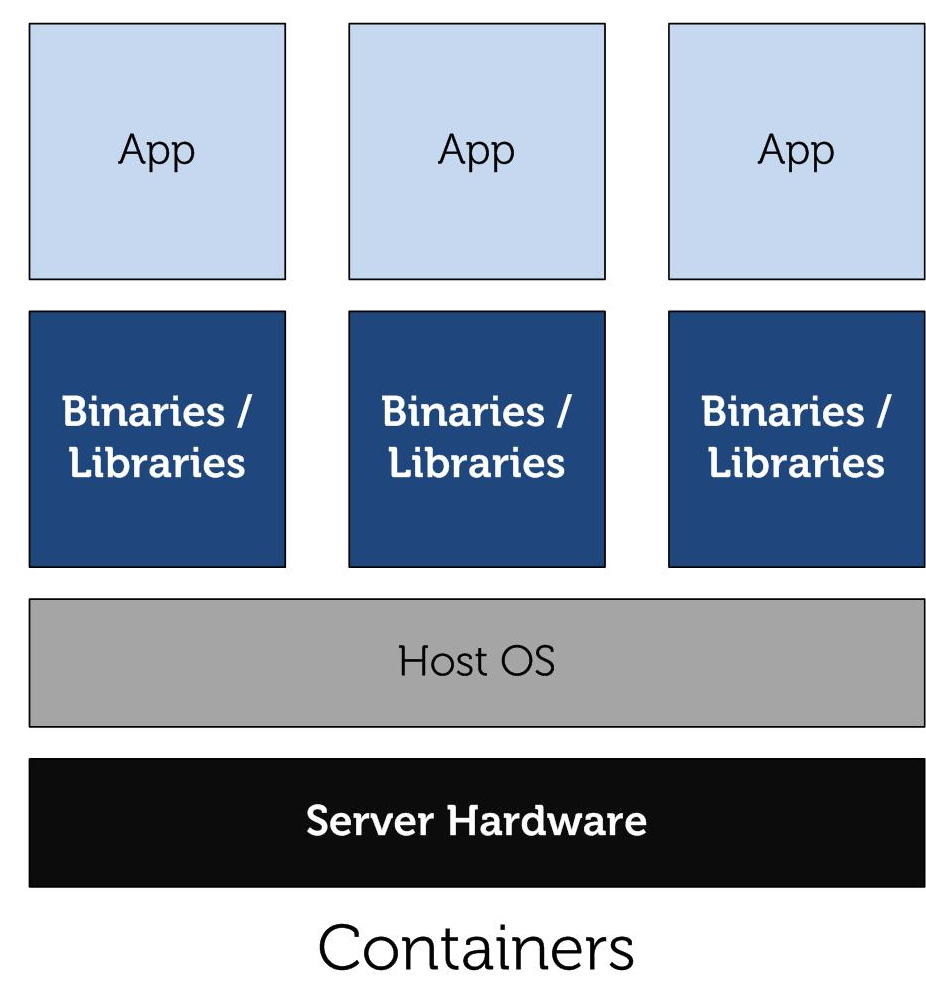
\includegraphics[width=0.5\textwidth]{Figures/containers.png}
    	\caption{Virtualización basada en contenedores: los contenedores comparten el sistema operativo del host y por lo tanto no necesitan una copia.}
    	\label{fig:contenedor-arch}
     \end{subfigure}
    ~ 
    \begin{subfigure}[b]{0.5\textwidth}
         \centering
    	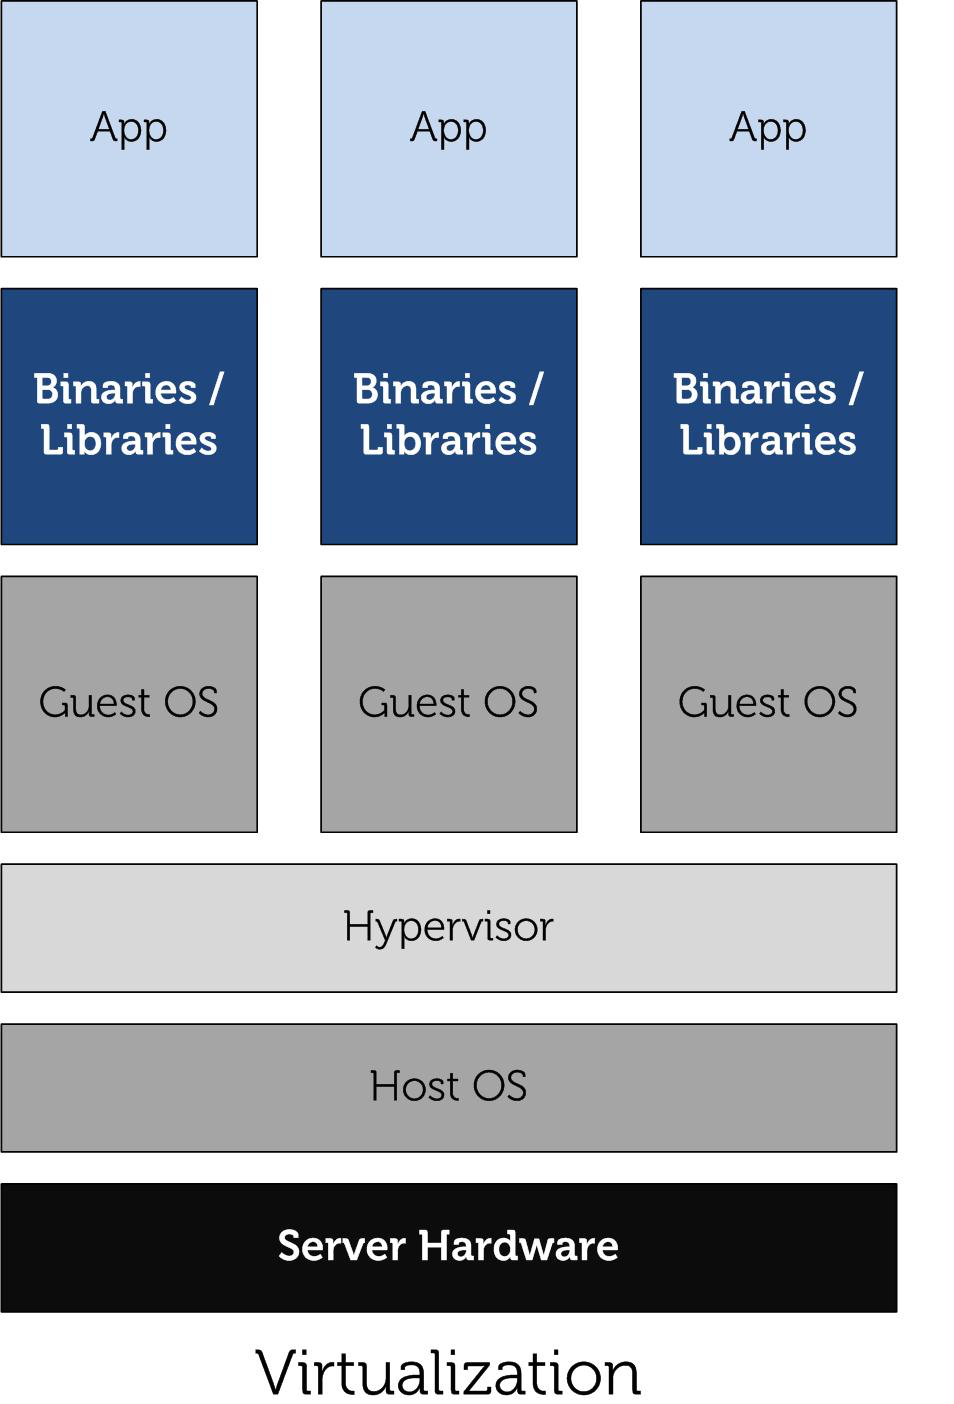
\includegraphics[width=0.5\textwidth]{Figures/virtual.png}
    	\caption{Virtualización basada en máquinas virtuales: las máquinas virtuales requieren un sistema operativo para cada uno.}
    	\label{fig:vm-arch}
     \end{subfigure}
        \caption{Dado que un contenedor comparte recursos, esto reduce significativamente el uso de almacenamiento en comparación a las máquinas virtuales.}
        \label{fig:dependencies-graph}
\end{figure*}

Las diferencias entre la virtualización basada en contenedores y máquinas virtuales presentan características interesantes para la ejecución de aplicaciones y workflows. Dado que un contenedor comparte recursos con el sistema operativo, como las bibliotecas, ésto reduce significativamente la necesidad de reproducir el código del sistema operativo, y significa que un servidor puede ejecutar varios ambientes con una sola instalación del sistema operativo. 
Por lo tanto, los contenedores son excepcionalmente ligeros: sólo tienen un tamaño de megabytes y sólo tardan unos segundos en arrancar. En comparación con los contenedores, las máquinas virtuales tardan minutos en funcionar y son un orden de magnitud mayor que un contenedor equivalente. \cite{padala2007performance,regola2010recommendations,felter2014updated}. A partir de esto nace la motivación de la utilización de contenedores con una alternativa para alcanzar la conservación física de los ambientes.
Docker es un proyecto open-source que utiliza la tecnología de los contenedores (libcontenedor) para ``construir, migrar y correr aplicaciones distribuidas". Actualmente utilizado por Yelp, Spotify, entre otros \cite{Docker:2015:Online, marmolnetworking}
Docker es una solución que simplifica el uso de los contenedores que han estado presente durante más de una década. Primero provee una interfaz simple y segura para crear y controlar contenedores \cite{bui2015analysis}, segundo permite a los desarrolladores empaquetar y correr sus aplicaciones de manera sencilla y además se integra con herramientas terceras que permiten administración y despliegue como Puppet\footnote{\url{https://puppet.com}}, Ansible \footnote{\url{https://ansible.com}} y Vagrant\footnote{\url{https://vagrant.com}}. Y diversas herramientas de orquestación como Mesos \cite{Apach91:online}, Shipyard \cite{shipy13:online}, Kubernetes \cite{kubernetes:2015:Online}, RancherOS \cite{Ranch38:online} y Docker Swarm	 \cite{Docke38:online}.

Docker puede separarse en dos grandes componentes Docker Engine y Client.
Docker Engine es una herramienta liviana y portable para administrar la virtualización. Y Docker Client, provee una interfaz para interactuar con los contenedores con los usuarios a través de RESTful APIs\cite{bui2015analysis}.\\

\begin{figure}[]
  \centering
    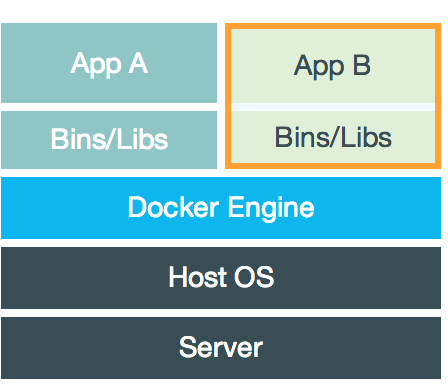
\includegraphics[width=0.3\textwidth]{Figures/docker.png}
    \caption{Docker}
    \label{fig:docker}
\end{figure}

Docker utiliza una arquitectura de cliente-servidor, Docker Client interactua con Docker Daemon y este construye, maneja y corre los contenedores. Docker Client y Docker Daemon pueden correr en el mismo host o se puede conectar el cliente desde un host remoto. El cliente y el Daemon se comunican en forma de sockets o RESTful API \cite{Docker:2015:understanding}.
Una imagen de Docker (\textit{Docker Image}) es una plantilla de solo lectura. Por ejemplo, una imagen puede contener las herramientas básicas de Ubuntu con Apache y una aplicación web instalada o simplemente el sistema operativo. Las imágenes son usadas para construir \emph{Docker contenedores}. Cuando el usuario crea cambios en el contenedor, este cambio no se realiza en la imagen, sino  que Docker añade una capa adicional con los cambios de la imagen\cite{bui2015analysis}. Por ejemplo, si el usuario utiliza una imagen base de Debian, luego añade el paquete emacs y luego añade el paquete apache, el estado de capas estaría representado por la figura \ref{fig:arquitectura} \cite{Docker:2015:Online}. Esto permite tener un proceso de distribución de imágenes más eficiente dado que solo es necesario distribuir las actualizaciones \cite{bui2015analysis}. El sistema de archivos descrito anteriormente se denomina una sistema de archivo basado en capas.
\begin{figure}[]
  \centering
  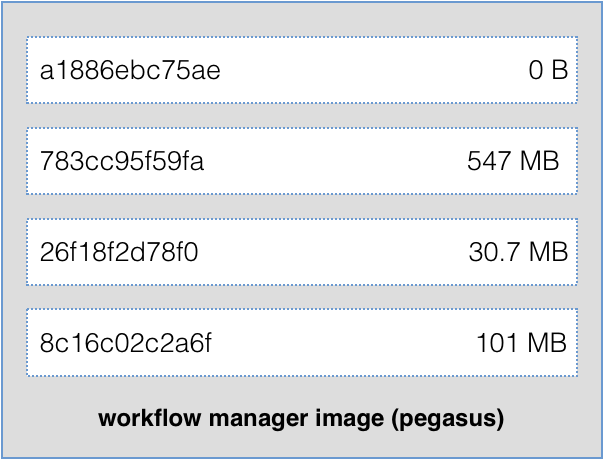
\includegraphics[width=0.6\textwidth]{Figures/docker-filesystems-multilayer}
    \caption{Las imágenes Docker con compuestas por capas. La última capa (a1886ebc75ae) es la única capa en modo escritura.}
    \label{fig:arquitectura}
\end{figure}	

Docker Hub es un repositorio que almacena dos tipos de repositorios públicos, oficiales y comunitarios. Los repositorios oficiales contienen imágenes públicas y verificadas de empresas y proveedores de software de renombre, como Canonical, Nginx, Red Hat y el propio Docker. Al mismo tiempo, los repositorios comunitarios pueden ser repositorios públicos o privados creados por usuarios y organizaciones individuales, que comparten sus aplicaciones y resultados. 

Usando ese repositorio y una línea de comandos, es posible descargar e implementar imágenes Docker localmente, ejecutando el contenedor en un entorno host, y ejecutando así el software dentro de la imagen. Los usuarios pueden crear y almacenar imágenes en el registro del Docker Hub, creando un archivo descriptor llamado Dockerfile o ampliando uno existente.  Este descriptor describe cuáles son los paquetes de software que estarán dentro de la imagen, construye la imagen y finalmente la sube al Docker Hub. Sin embargo, Docker Hub no controla qué paquetes hay en las imágenes, si la imagen se desplegará correctamente o si las imágenes pueden tener algún problema de seguridad. 
Así, las imágenes Docker funcionan como una caja negra, lo que significa que los usuarios saben sólo paquetes principales que se ejecutan dentro del contenedor pero no conocen los otros paquetes necesarios para ejecutarlo.
Hay dos maneras de subir imágenes a un repositorio de usuario, ya sea enviar la imagen desde un host local o automatizando ese proceso desde un repositorio Github. Para enviar una imagen al Docker Hub, los usuarios necesitan nombrar sus imágenes locales usando su nombre de usuario Docker Hub, y el nombre del repositorio que han creado. Después, los usuarios añaden múltiples imágenes a un repositorio añadiéndole la versión \texttt{:<tag>}. Esta es toda la información que normalmente tienen las imágenes Docker en DockerHub, siendo por tanto casi imposible reproducir el entorno de ejecución si se modifica alguno de los paquetes de software utilizados dentro de las imágenes. 
 
 
DockerHub permite a las comunidades científicas almacenar y compartir, conservando el contenido de los contenedores, así como comprobar la identidad del editor y recuperar los contenedores de interés. Sin embargo, la información del contenido de cada repositorio no siempre es accesible de forma clara. 
Como la mayoría de las veces sólo se proporcionan descripciones cortas de los contenedores, no es fácil para el usuario entender qué componentes están instalados en ellos. 
Incluso cuando los archivos Dockerfile están disponibles, no son lo suficientemente intuitivos de entender cuáles paquetes están siendo desplegados por cada comando.
Además, es posible que en el contenedor existan algunos componentes que no estén especificados por el propio Dockerfile. Para abordar este problema proponemos un enfoque automático para analizar el contenido de un contenedor Docker y extraer la información sobre los componentes de software instalados en él. Esta información se convierte en datos semánticos, codificados como RDF bajo el conjunto de ontologías.

Los contenedores Docker consiste de un ambiente virtual con: con archivos de usuarios y metadata, cada contenedor es construido a partir de una imagen base como se mencionó anteriormente. 
Esta imagen indica la base del contenedor y se asocia un proceso inicial, él cual debe correr cuando el contenedor es iniciado~\cite{Docker:2015:understanding}. Para describir los pasos incluidos en la creación de un contenedor, se ejemplificará con la creación de uno.

\begin{figure*}
	\begin{lstlisting}[caption={Ejemplo de la ejecutación de un contenedor utilizando la imagen Docker},label={lst:tensorflow},language=bash]
	docker run -i -t ubuntu /bin/bash
\end{lstlisting}
\end{figure*}

	\begin{itemize}
		\item \emph{Docker Client} le informa al Docker que debe correr un contenedor.
		\item En este caso el comando \texttt{/bin/bash} será el proceso \texttt{init} o 0 del contenedor
		\item \textbf{Traer la imagen:} Docker verifica la existencia de la imagen Ubuntu y sino existe en el host, entonces Docker descarga desde el repositorio ya sea privado o publico. Si la imagen existe entonces crea el contenedor.
		\item \textbf{Asignar el sistema de archivos y montar la capa de escritura:} El contenedor es creado en el sistema de archivos y se añade una capa en modo escritura en la imagen.
		\item \textbf{Crear la red y conectar con la interfaz puente:} Crea la interfaz de red que permite que contenedor pueda enviar y recibir paquetes con el host a través del puente (docker0).
		\item \textbf{Asignar un IP:} Asigna una dirección IP del pool al contenedor
		\item \textbf{Capturar la salida estándar y de errores:} Dependiendo de la configuración de contenedor, Docker enviará a los registros de errores hacia el mismo servidor u otro externo.
	\end{itemize}

Docker utiliza dos funcionalidades de Linux \emph{namespaces} y \emph{cgroups} para crear ambientes virtuales para los contenedores. \emph{cgroups} o \emph{control groups} proveen un mecanismo de contabilidad y limites de recursos que pueden utilizar los contenedores\cite{bui2015analysis}. Los \emph{namespaces} proveen del aislamiento que es llamado contenedor. 
Cuando sea crea un contenedor, Docker crea un conjunto de \emph{namespaces} para el contenedor. Los \emph{namespaces} utilizados por Docker: mount (mnt) para el manejo del montaje, PID para el aislamiento de los procesos, net para el manejo de interfaces y IPC para acceder a recursos de IPC. 
Docker logra el aislamiento de los procesos separando los procesos en \emph{namespaces} y limitando los permisos de los procesos a otros contenedores. 
\emph{PID namespaces} (añadido en el kernel \( \geq 2.6.3.2)\) es el mecanismo utilizado, logrando que un proceso que se encuentra en el contenedor solo pueda ver procesos que se encuentra en ese contenedor. Por lo tanto un atacante no puede observar procesos de otro contenedor, lo que aísla al contenedor este nivel \cite{bui2015analysis, LVM:2015:Online}.
Docker usa \emph{mount namespaces} o \emph{filesystem namespaces} para aislar los \emph{filesystems} asociados a los contenedores. De la misma forma que ocurre con los procesos, los eventos del sistema de archivo que ocurre en el contenedor sólo afectan a ese contenedor.

Cómo se menciono anteriormente, Docker utiliza \emph{cgroups} que permite especificar que \emph{device} puede ser utilizado con el contenedor. Esto bloquea la posibilidad de crear y usar \emph{device nodes} que puedan ser utilizados para atacar el host. Los \emph{device nodes} que son creados para cada contenedor por defecto: son: /dev/console, /dev/null, /dev/zero, /dev/full, /dev/tty*, /dev/urandom, /dev/random, /dev/fuse. \cite{walsh:2014:Online}
IPC (\emph{inter-process communication} es un conjunto de objetos para el intercambio de datos a través de los procesos, como semáforos, colas de mensajes, segmentos de memoria compartida. Los procesos corriendo en los contenedores utilizan \emph{IPC namespaces} que permite la creación de un \emph{IPC} separado y independiente para cada contenedor, con esto se previene que procesos en un contenedor interfieran con otros contenedores o el host.
Para cada contenedor, Docker crea una red independiente usando \emph{network namespaces}, compuesta de su propia IP, rutas, \emph{network devices}. Esto permite que el contenedor pueda interactuar con otro host a través de su propia interfaz.
Por omisión, la conexión se realiza gracias al host que provee un \emph{Virtual Ethernet bridge} en la máquina host, llamado docker0 que automáticamente realiza un \emph{forward} de los paquetes entre las interfaces. Cuando Docker crea un nuevo contenedor, esto establece una interfaz de red virtual con un nombre único que se conecta con el \emph{bridge (docker0)} y con la interfaz \emph{eth0} del contenedor \cite{bui2015analysis}.
Además para controlan la cantidad de recursos como CPU, memoria, \emph{disk I/O} que el contenedor puede utilizar se utiliza \emph{Cgroups}. A partir de esto se protege contra ataques de DoS.


\section{Web Semantica}

La web semántica es un extensión \emph{World Wide Web} añadiendo un conjunto de estándares  diseñado por la \emph{World Wide Web Consortium} con el objetivo de la creación de tecnologías para publicar datos legibles por aplicaciones informáticas. Para lo lograr lo anterior, se añaden metadatos semánticos y ontologías para describir el contenido y generar relaciones entre los datos, esta representación se realiza de una manera formal.
Consecuentemente, la información disponible pueden ser procesadas de manera automática mejorando la inter operatividad  entre distintos sistemas informáticos que realizan búsquedas sin operadores humanos.

El término fue acuñado por Tim Berners-Lee para una red de datos que puede ser procesada por máquinas es decir, una red en la que gran parte del significado es legible por máquinas. En \cite{berners1992world} se afirma la necesidad de que los datos se transformen desde objetos legible por personas a información semántica diseñada para las máquinas.

Es por ello que la web semántica ha definido diversos estándares para construir una descripción formal de los conceptos, términos y relaciones.  Estos estándares definidos por W3C incluyen: RDF, RDFS, SPARQL, Notation3 (N3), N-Triples, Turtle y OWL.

% Para lograr los objetivos de la Web Semántica se han generado múltiples estándares de representación como son XML, XML Schema, RDF, RDF Schema, OWL y SPARQL.

\subsection{RDF}\label{sw:rdf}
RDF (del inglés \emph{Resource Description Framework}) es una familia de
especificaciones del W3C diseñada como un modelo de datos para metadatos.
Fue adoptado como una recomendación del W3C en 1999, mientras que la
especificación 1.0 fue publicada el 2004 y la 1.1 el
2014\cite{bikakis2013semantic}.

El modelo de datos RDF se basa en la idea de hacer declaraciones sobre 
recursos Web (URIs) en forma de expresiones $\langle sujeto, predicado, objeto
\rangle$ que son llamados triples RDF.
El $sujeto$ indica el recurso mientras que el $predicado$ denota la relación de
éste con el $objeto$.
Así podemos decir que un triple RDF sigue la clásica notación \tt{entidad} - 
\tt{atributo} - \tt{valor} de los modelos orientados a objetos, permitiendo
además, gracias a su simpleza, modelar todo tipo de conceptos abstractos.

\subsection{RDFS}
RDFS (de las siglas del íngles \emph{Resource Description Framework Schema},
también llamado RDF Schema) es un vocabulario que extiende RDF proveyendo un
set de clases y propiedades que mejoran la creación de modelos como son:
\tt{Class} para declarar clases, \tt{subClassOf} para denotar herencia,
\tt{range} y \tt{domain} para el rango y dominio de cierta propiedad
(\tt{rdf:Property}), entre otras.

RDF fue presentado en 1998 e introducido finalmente como recomendación del W3C
el 2004\cite{bikakis2013semantic}.

\subsection{OWL}
OWL (del íngles \emph{Web Ontology Language}) es una familia de lenguajes para
la creación de ontologías complejas.
Agrega lógica computacional para que las relaciones
hechas con este lenguaje puedan ser procesadas con el fin de verificar la
consistencia de la información o generar información implicita.

La versión actual de OWL se conoce como ``OWL 2'' y fue publicada el 2009 como 
una revisión y extensión de la versión inicial publicada el
2004\cite{bikakis2013semantic}. Generalmente cuando se habla de ``OWL'' nos
referimos a la versión del 2004.


\section{Sistemas de paquetes y vulnerabilidades}


